\documentclass[11pt, oneside]{article}   	% use "amsart" instead of "article" for AMSLaTeX format


%\usepackage{draftwatermark}
% \SetWatermarkText{Confidential}
% \SetWatermarkScale{5}
% \SetWatermarkLightness {0.85} 
% \SetWatermarkColor[rgb]{0.7,0,0}


\usepackage{geometry}                		% See geometry.pdf to learn the layout options. There are lots.
\geometry{letterpaper}                   		% ... or a4paper or a5paper or ... 
%\geometry{landscape}                		% Activate for for rotated page geometry
%\usepackage[parfill]{parskip}    		% Activate to begin paragraphs with an empty line rather than an indent
\usepackage{graphicx}				% Use pdf, png, jpg, or eps� with pdflatex; use eps in DVI mode
								% TeX will automatically convert eps --> pdf in pdflatex		
\usepackage{amssymb}
\usepackage{hyperref}
\usepackage{url}
\usepackage{authblk}
\usepackage{amsmath}
\usepackage{graphicx}
\usepackage{fixltx2e}
\usepackage{hyperref}
\usepackage{alltt}
\usepackage{color}
\usepackage{dsfont}


\title{How exactly does word2vec work?}
\author{David Meyer \\ dmm@\{1-4-5.net,uoregon.edu,brocade.com,...\}}
% \date{June 17, 2015}							% Activate to display a given date or no date


\begin{document}
\maketitle

\section{Introduction} 
\label{sec:intro}
The word2vec model \cite{Mikolov2014} and its applications have recently attracted a great deal of attention from the machine learning community. These \emph{dense vector representations} of words learned by word2vec have remarkably been shown to carry semantic meanings and are useful in a wide range of use cases ranging from natural language processing to network flow data analysis.

\bigskip
\noindent
Perhaps the most  amazing property of these word embeddings is that somehow these vector encodings effectively capture the semantic meanings of the words. The question one might ask is how or why?  The answer is that because the vectors adhere surprisingly well to our intuition. For instance, words that we know to be synonyms tend to have similar vectors in terms of cosine similarity and antonyms tend to have dissimilar vectors. Even more surprisingly, word vectors tend to obey the laws of analogy. For example, consider the analogy "Woman is to queen as man is to king". It turns out that
\begin{center}
$v_{\text{queen}} -  v_{\text{woman}} + v_{\text{man}} \approx v_{\text{king}}$
\end{center}

\noindent
where $v_{\text{queen}}, v_{\text{woman}} ,v_{\text{man}}$ and $ v_{\text{king}}$ are the word vectors for queen, woman, man, and king respectively. These observations strongly suggest that word vectors encode valuable semantic information about the words that they represent.


\bigskip
\noindent
Note that there are two main word2vec models: Continuous Bag of Words (CBOW) and Skip-Gram. In the CBOW model, we predict a word given a context (a context can be something like a sentence).  Skip-Gram is the opposite: predict the context given an input word. Each of these models is examined below.

\bigskip
\noindent
This document contains my notes on the word2vec. NB: there are probably lots of mistakes in this...

\section{Continuous Bag-of-Words Model}

The simplest version of the continuous bag-of-word model (CBOW) is a "single context word" version \cite{Mikolov:2013aa}. This is  shown in Figure \ref{fig:simple_cbow}. Here we assume that there is only one word considered per context, which means the model will predict one target word given one context word (which is similar to a bi-gram language model).

\begin{figure}
\center{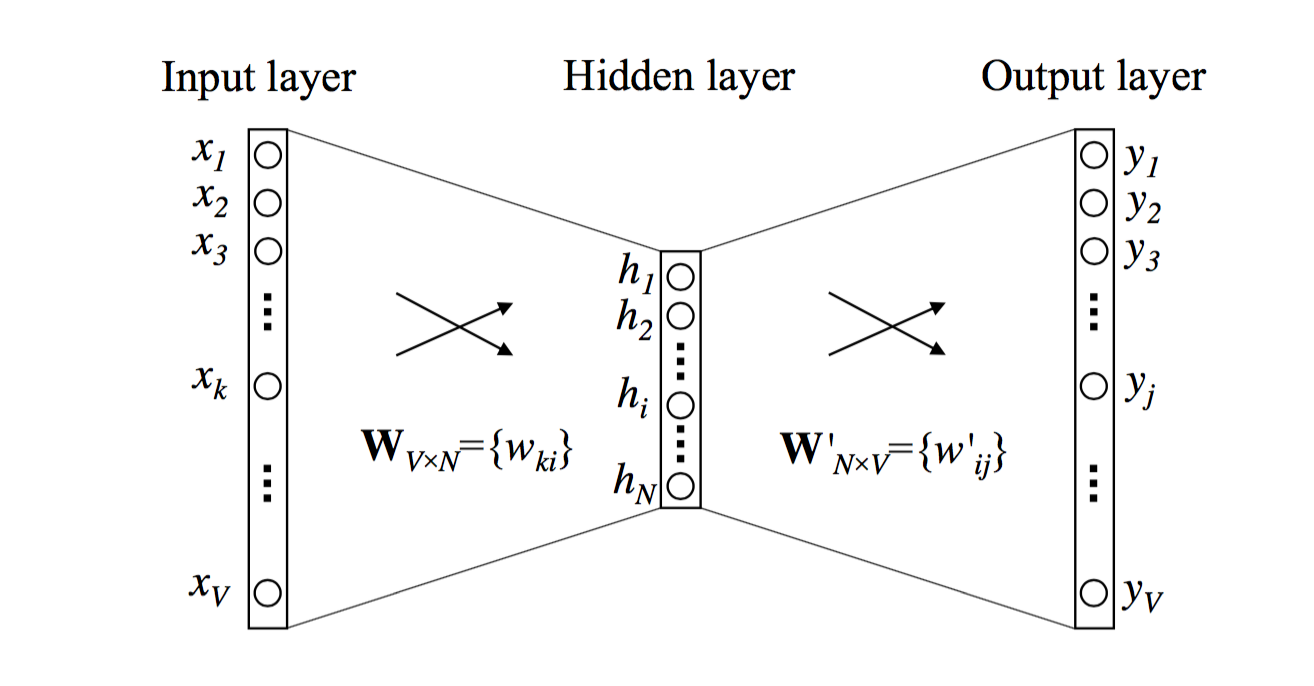
\includegraphics[scale=0.4]{images/simple_cbow.png}}
\caption{Simple CBOW Model}
\label{fig:simple_cbow}
\end{figure}

\bigskip
\noindent
In the scenario depicted in Figure \ref{fig:simple_cbow}, $V$ is the vocabulary size and the hyper-parameter $N$ is the hidden layer size. The input vector $\mathbf{x} = \{x_{1}, x_{2},\hdots,x_{V}\}$ is one-hot encoded, that is,  that some $x_{k} =1$ and  all other $x_{k^\prime} = 0$ for $k \neq k^\prime$.

\bigskip
\noindent
The weights between between the input layer and the hidden layer can be represented by the $V \times N$ matrix \textbf{W}. Each row of \textbf{W} is the $N$-dimensional vector representation $\mathbf{v}_{w}$ of the associated word $w$ in the input layer. Give a context (here a single word), and assuming again $x_{k} = 1$ and $x_{k^\prime} = 0$ for  $k \neq k^{\prime}$ (one-hot encoding), then
\begin{flalign}
\mathbf{h} = \mathbf{x}^{\text{T}}\mathbf{W} = \mathbf{W}_{(k,.)} := \mathbf{v}_{w_I}
\label{eqn:h}
\end{flalign}
 
\noindent
This essentially copies the $k$-th row of \textbf{W} to \textbf{h} (this is due to the one-hot encoding 
of \textbf{x}). Here $\textbf{v}_{w_{I}}$ is the vector representation of the input word $w_{I}$. Note that this implies that the link (aka activation) function of the hidden units is linear ($g(x) = x$). Recall that

\begin{flalign}
 \mathbf{W}_{V\times N} &= 
 \begin{bmatrix}
w_{\text{\tiny{11}}}  & w_{\text{\tiny{12}}}   & \dots    & w_{\text{\tiny{1N}}}   \\
w_{\text{\tiny{21}}}  & w_{\text{\tiny{22}}}   & \dots    & w_{\text{\tiny{2N}}}   \\
\vdots                      & \vdots                      & \ddots  & \vdots                        \\
w_{\text{\tiny{V1}}}  & w_{\text{\tiny{V2}}}  & \dots    & w_{\text {\tiny{VN}}}
\end{bmatrix}
\end{flalign}

\bigskip
\noindent
and

\begin{flalign}
\boldsymbol{x} & = \begin{bmatrix}  x_{1}         \\  
                                                         x_{2}         \\ 
                                                         \vdots        \\  
                                                         x_{\text{\tiny{V} }}        
                                \end{bmatrix} 
\end{flalign}

\noindent
so that 

\begin{flalign}
\mathbf{h} & = \mathbf{x}^{\text{T}}\mathbf{W} = \begin{bmatrix}  x_{1} \:  x_{2} \:  \hdots \:  x_{\text{\tiny{k}}} \: \hdots \:x_{\text{\tiny{V}}}  
\end{bmatrix}
\begin{bmatrix}
w_{\text{\tiny{11}}}  & w_{\text{\tiny{12}}}    & \dots     & w_{\text{\tiny{1N}}}    \\
w_{\text{\tiny{21}}}  & w_{\text{\tiny{22}}}    & \dots     & w_{\text{\tiny{2N}}}    \\
\vdots                      & \vdots                       & \ddots   & \vdots                         \\
w_{\text{\tiny{k1}}}  & w_{\text{\tiny{k2}}}    & \hdots   & w_{\text{\tiny{kN}}}     \\
\vdots                      & \vdots                       & \ddots   & \vdots                         \\
w_{\text{\tiny{V1}}}  & w_{\text{\tiny{V2}}}   & \dots     & w_{\text {\tiny{VN}}}   \\
\end{bmatrix} \\
&= \begin{bmatrix}
x_{k}w_{\text\tiny{k1}}  \  x_{k}w_{\text{\tiny{k2}}}  \ \hdots \  x_{k}w_{\text{\tiny{kN}}} 
\end{bmatrix}    \qquad \text{\text{\#} for $x_{k} = 1, x_{k^\prime} = 0 \: \text{for} \: k \neq k^\prime$} \\
&= \begin{bmatrix}
w_{\text\tiny{k1}} \  w_{\text{\tiny{k2}}}  \ \hdots \ w_{\text{\tiny{kN}}} 
\end{bmatrix}   \quad  \qquad \qquad \text{\text{\#} $k$-th row of \textbf{W}} \\
&= \mathbf{W}_{(k,.)} \\
& := \mathbf{v}_{\text{\tiny{WI}}}
\end{flalign}

\bigskip
\noindent
From the hidden layer to the output layer there is a different weight matrix 
$\textbf{W}^{\prime} = \{w^{\prime}_{i,j}\}$ which is a $N \times V$ matrix. Using this we can compute a score for 
each word in the vocabulary: 

\begin{flalign}
 u_j = {\mathbf{v}^{\prime}_{w_j}}^{\text{T}}  \cdot \mathbf{h}
 \label{eqn:u_sub_j}
\end{flalign}

\noindent
where $\mathbf{v}^{\prime}_{w_j}$ is the $j$-th column of the matrix $\mathbf{W}^\prime$. 
Note that the score $u_j$ is a measure of the match between the context and the next word
\footnote{Though almost all statistical language models predict the next word, it is also possible to model the distribution of the word preceding the context or surrounded by the context.}
 and is computed by taking the dot product between the predicted representation ($\mathbf{v}^{\prime}_{w_j}$) and the representation of the candidate target word ($\mathbf{h} = \mathbf{v}_{wI}$).

\bigskip
\noindent
Now you can use a softmax (log linear) classification model to obtain the posterior distribution of words (turns out to be multinomial distribution):

\begin{flalign}
p(w_{j} | w_{I}) = y_{j} = \frac{exp(u_{j})}{\sum\limits_{j^{\prime} = 1}^{V} exp(u_{j^\prime})}
\label{eqn:posterior}
\end{flalign}

\noindent
where $y_j$ is the output of the $j$-th unit of the output layer. Substituting Equations  \ref{eqn:h} and \ref{eqn:u_sub_j} into Equation \ref{eqn:posterior} we get

\begin{flalign}
p(w_{j} | w_{I}) = \frac{exp\big({\mathbf{v}^{\prime}_{wo}}^{\text{T}} \mathbf{v}_{w_I}\big)}
{\sum\limits_{j^{\prime} = 1}^{V} exp\big ({\mathbf{v}^{\prime}_{w_{j}^{\prime}}}^{\text{T}}\mathbf{v}_{wI}\big)}
\label{eqn:sub_posterior}
\end{flalign}

\noindent
Notes

\begin{itemize}
\item{Both the input vector \textbf{x} and the output \textbf{y} are one-hot encoded}
\item{$v_{w}$ and $v^{\prime}_w$ are two representations of the input word $w$}
\item{$v_{w}$ comes from the rows of \textbf{W}}
\item{$v_{w}^\prime$ comes from the columns of $\textbf{W}^{\prime}$}
\item{$v_{w}$ is usually called the \emph{input vector}}
\item{$v_{w}^\prime$ is usually called the \emph{output vector}}
\end{itemize}

\subsection{Updating Weights: hidden layer to output layer}
\label{sec:hidden_to_output}

The training objective (for one training sample) is to maximize Equation \ref{eqn:sub_posterior}, the conditional probability of observing the actual output word $w_O$ (denote its index in the output layer as $j^*$) given the input context word $w_I$  (and with regard to the weights). That is,

\begin{flalign}
\text{max } p(w_{\text{\tiny{O}}} | w_{\text{\tiny{I}}}) &= \text{max } y_{j^*}       \\
                                                                                 &= \text{max} \log y_{j^*} \\
                                                                                 &= u_{j^*} - \log \sum\limits_{j^\prime = 1}^{V} exp(u_{j^\prime}) := - E
\end{flalign}

\noindent
where $E = - \log  p(w_{\text{\tiny{O}}} | w_{\text{\tiny{I}}})$ is our loss function (which we want to minimize), 
and $j^*$ is the index of the actual output word (in the output layer). Note (again) that this loss function can be understood as a special case of the cross-entropy measurement between two probabilistic distributions.

\bigskip
\noindent
The next step is to derive the update equation of the weights between hidden and output layers. Take 
the derivative of $E$ with respect to $j$-th unit's net input $u_j$, we obtain

\begin{flalign}
\frac{\partial E}{\partial u_j} & = y_j -t_j  := e_j
\label{eqn:E}
\end{flalign}
\noindent
where $t_j = \mathds{1}(j = j^{*})$, the indicator function, i.e., $t_j$ will be 1 when the $j$-th unit 
is the actual output word, otherwise  $t_j = 0$ . Interestingly this derivative is simply the prediction 
error $e_j$ of the output layer. 

\bigskip
\noindent
The next step is to  take the derivative on $w^{\prime}_{ij}$ to obtain the gradient on the
$\text{hidden} \rightarrow \text{output}$ weights which (by the chain rule) is
\bigskip
\begin{flalign}
\frac{\partial E}{\partial w^{\prime}_{ij}} = \frac{\partial E}{\partial u_j} \cdot \frac{\partial u_j}{\partial w^{\prime}_{ij}} = e_j \cdot h_i
\end{flalign}
\noindent
since (sketch of the proof)
\begin{flalign}
\frac{\partial E}{\partial u_j}  
&= \frac{\partial \bigg (u_{j^*} - \log \sum\limits_{j^\prime = 1}^{V} exp(u_{j^\prime}) \bigg )} {\partial u_{j^*}} \\
&= \frac{\partial u_{j^{*}}}{\partial u_j} - \frac{\partial \bigg ( \log \sum\limits_{j^\prime = 1}^{V} exp(u_{j^\prime}) \bigg )}{\partial u_j} \\
&= t_j - \frac{exp(u_j)}{ \sum\limits_{j^\prime = 1}^{V} exp(u_{j^\prime})} \\
&= t_j - y_j \quad \qquad \qquad \qquad \text{\# by Equations \ref{eqn:posterior} and \ref{eqn:E}}
\end{flalign}

\bigskip
\noindent
Now, using stochastic gradient descent, we obtain the weight updating equation for 
$\text{hidden} \rightarrow \text{output}$ weights:

\begin{flalign}
w{^{\prime}_{ij}}^{\text{(new)}} = w{^{\prime}_{ij}}^{\text{(old)}} - \eta \cdot e_j \cdot h_i
\end{flalign}
 
 \noindent
 and/or 
 
\begin{flalign}
\mathbf{v}{{^\prime}_{w_j}}^{\text{(new)}} = \mathbf{v}{{^\prime}_{w_j}}^{\text{(old)}} - \eta \cdot e_j \cdot \mathbf{h}
\end{flalign}

\bigskip
\noindent
where $\eta > 0$ is the learning rate (standard SGD), $e_j = y_j -t_j$ (Equation \ref{eqn:E}), $h_i$ is the $i$-th unit in the hidden layer, and $\mathbf{v}{{^\prime}_{w_j}}$ is the output vector for word $w_j$.

\subsection{Updating Weights: Input to hidden layers}
Now that we have the update equations for $\mathbf{W}^{\prime}$, we an look at \textbf{W}. Here we take the derivative for $E$ on the output of the hidden layer:

\begin{flalign}
\frac{\partial E}{\partial{h_i}} &= \sum\limits_{j = 1}^{V} \frac{\partial E}{\partial u_j} \cdot \frac{\partial u_j}{\partial h_i} \\
&= \sum\limits_{j = 1}^{V} e_j \cdot w^{\prime}_{ij} \\
& := \text{EH}_{i}
\end{flalign}
\noindent
where $h_i$ is the output of the $i$-th unit in the hidden layer, $u_j$ is defined in Equation \ref{eqn:u_sub_j} (the input of the $j$-th unit to the output layer), and $e_j = y_j - t_j$ is the prediction error of the $j$-th word in the output layer. 
EH is an $N$-dimensional vector is the sum of the output vectors of all words in the vocabulary, weighted by their prediction error $e_j$. 

\bigskip
\noindent
The next job is to take the derivative of $E$ with respect to \textbf{W}. So first recall that the hidden layer performs a linear computation on the values from the input layer, specifically
\begin{flalign}
h_i  &= \sum\limits_{k = 1}^{V} x_k \cdot w_{ki} \qquad \qquad \text{\# see Equation \ref{eqn:h}}
\end{flalign}

\noindent
Now we can use the chain rule to get the derivative of $E$ with respect to \textbf{W}, as follows (chain rule again):
\begin{flalign}
\frac{\partial E}{\partial w_{ki}}  &= \frac{\partial E}{\partial h_{i}} \cdot \frac{\partial h_i}{\partial w_{ki}} \\
&= \text{EH}_i \cdot x_k 
\end{flalign}

\noindent
and so (vector form)
\begin{flalign}
\frac{\partial E}{\partial \mathbf{W}} &= \text{EH}  \cdot \mathbf{x}
\end{flalign}

\noindent
From this we obain an $V \times N$ matrix. Notice that since only one component of \textbf{x} is non-zero, only one row of $\frac{\partial E}{\partial \mathbf{W}}$ is non-zero, and the value of that row is EH (an $1 \times N$ dimensional vector).

\bigskip
\noindent
Now we can write the update equation for \textbf{W} as

\begin{flalign}
\mathbf{v}{{^\prime}_{w_I}}^{\text{(new)}} = \mathbf{v}{{^\prime}_{w_I}}^{\text{(old)}} - \eta \cdot \text{EH}
\label{eqn:v_update}
\end{flalign}

\noindent
Here $\mathbf{v_{w_I}}$ is a row of \textbf{W} (namely the input vector of the (only) context word), and because of the one-hot encoding it is the only row of \textbf{W} whose derivative is non-zero.


\section{General Continuous Bag-of-Words Model}

\begin{figure}
\center{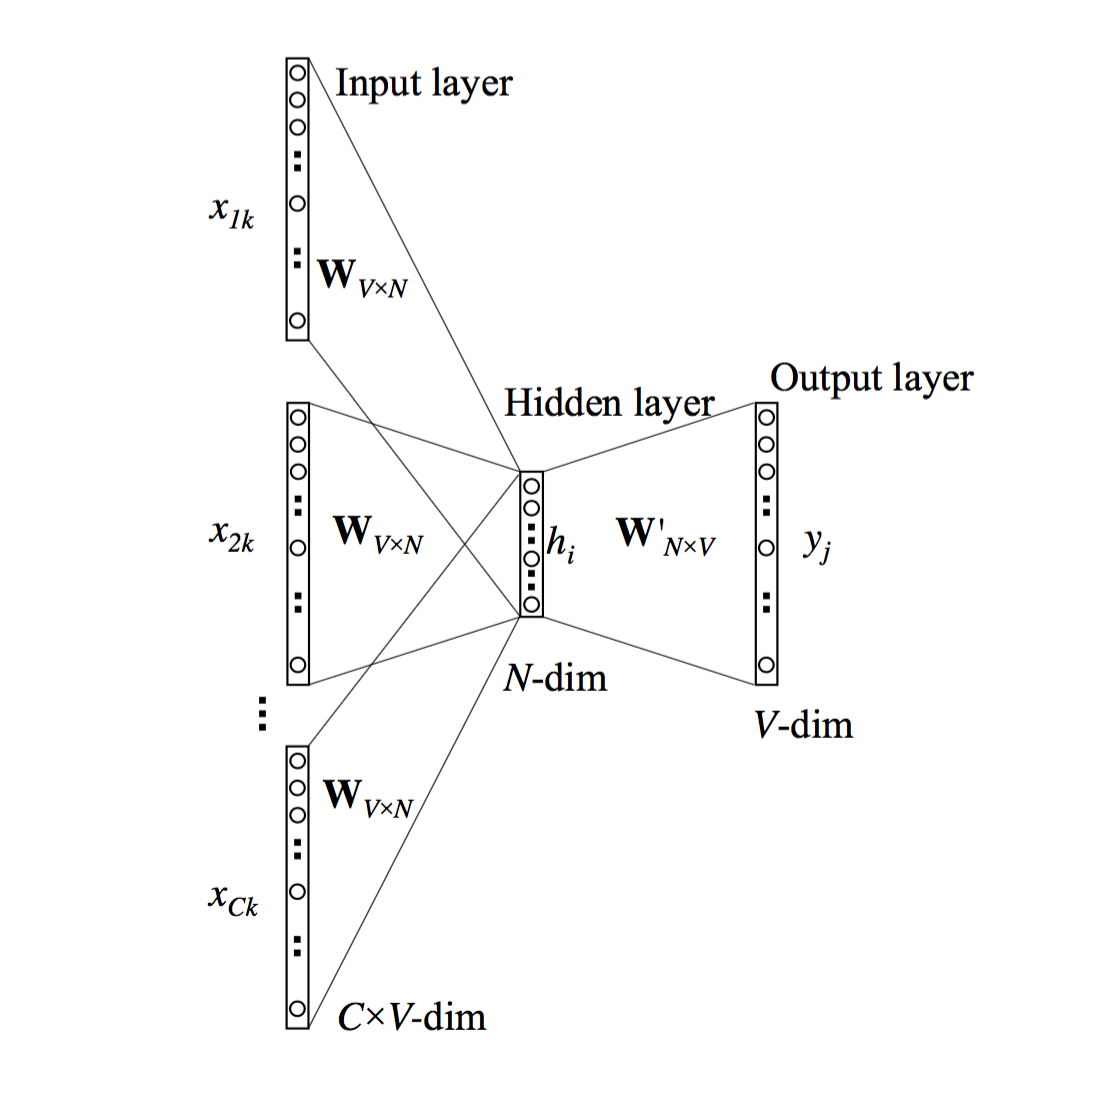
\includegraphics[scale=0.4]{images/full_cbow.png}}
\caption{General CBOW Model}
\label{fig:full_cbow}
\end{figure}


\section{Skip-Gram Model}

The Skip-Gram model was introduced in Mikolov \cite{Mikolov:2013aa} and is depicted in Figure \ref{fig:skip_gram}. As you can see, Skip-Gram is the opposite of CBOW; in Skip-Gram we predict the context $C$ given and input word, where is in CBOW we predict the word from $C$. Basically the training objective of the Skip-Gram model is to learn word vector representations that are good at predicting nearby words in the associated context(s).

\begin{figure}
\center{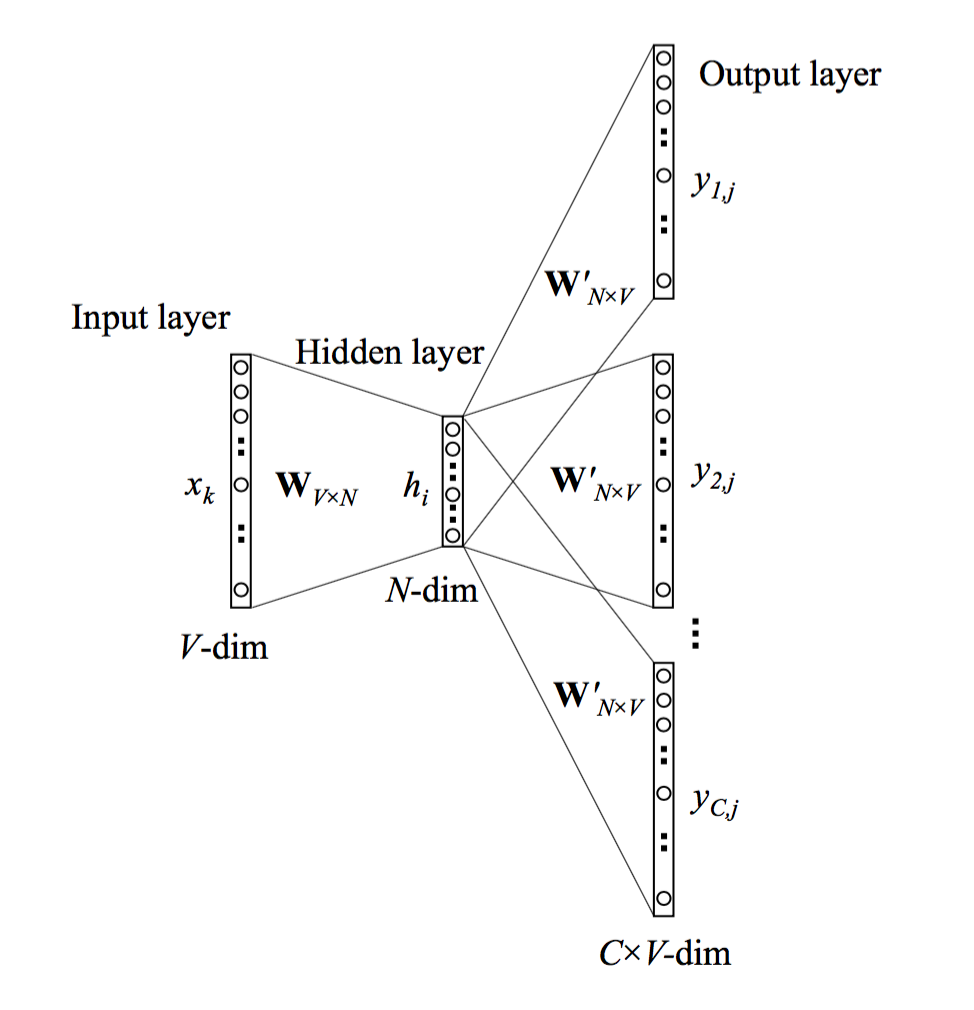
\includegraphics[scale=0.4]{images/skip_gram.png}}
\caption{Skip-Gram Model}
\label{fig:skip_gram}
\end{figure}

\bigskip
\noindent
For the Skip-Gram model we continue to use  $w_{w_i}$ to denote the input vector of the only word on the input layer, and as a result have the same definition of the hidden-layer outputs $h$ as in Equation \ref{eqn:h} (again this means $h$ copies a row from the $\text{input} \rightarrow \text{hidden}$ weight matrix $\mathbf{W}$ associated with input word $w_I$). Recall that the definition of $\mathbf{h}$ was 
\begin{flalign}
\mathbf{h} = \mathbf{W}_{(k,.)} := v_{\text{\tiny{wI}}}
\end{flalign}

\noindent
Now, at the output layer, instead of outputting one multinomial distribution, we output $C$ multinomial distributions. Each output is computed using the same $\text{hidden} \rightarrow \text{output}$ matrix as follows:

\begin{flalign}
\label{eqn:sg-posterior}
p(w_{\text{\tiny{c,j}}} = w_{\text{\tiny{O,c}}} | w_{\text{\tiny{I}}})  = y_{\text{c,j}} = \frac{exp(u_{\text{\tiny{c,j}}})}{\sum\limits_{j^{\prime }= 1}^{V} exp(u_{j^\prime})}
\end{flalign}

\noindent
where $w_{\text{\tiny{c,j}}}$ is the $j\text{-th}$ word on the $c\text{-th}$ panel of the output layer. $w_{\text\tiny{O,c}}$ is the actual $c\text{-th}$ word in the output context. Note that $w_{\text{\tiny{I}}}$ is the (only) input word. $y_{\text\tiny{c,j}}$ is the output of the $j\text{-th}$ unit on the $c\text{-th}$ panel of the output layer. Finally, $u_{\text{\tiny{c,j}}}$ is the input of the $j\text{-th}$ unit on the $c\text{-th}$ panel of the output layer. 

\bigskip
\noindent
Said in words, this is the probability that our prediction of the $j\text{-th}$ word on the $c\text{-th}$ panel, $w_{cj}$, equals the actual $c\text{-th}$ output word, $w_{\text{Oc}}$, conditioned on the input word $w_{\text{I}}$.

\bigskip
\noindent
Now, because the output layer panels share the same weights, we have
\begin{flalign}
u_{\text{\tiny{c,j}}} = u_{\text{\tiny{c}}} = {\mathbf{v}^{\prime}_{w_j}}^{T} \cdot \mathbf{h}\text{,} \:\; \text{for } c = 1, 2, \hdots, C
\end{flalign}

\noindent
where $\mathbf{v}^{\prime}_{w_j}$ is the output vector of the $j\text{-th}$ word $w_j$ of the 
vocabulary\footnote{$\mathbf{v}^{\prime}_{w_j}$ is again a column of the $\text{hidden} \rightarrow \text{output}$ weight matrix $\mathbf{W}^{\prime}$}.

\bigskip
\noindent
Given all of this, the parameter update equations are not so different from the one context word
CBOW model. The loss function is changed to

\begin{flalign}
\label{eqn:negative_log_likelihood}
E & = - \log p(w_{\text{\tiny{O,1}}}, w_{\text{\tiny{O,2}}}, \hdots, w_{\text{\tiny{0,C}}} | w_{\text{\tiny{I}}}) \\
   & = - \log \prod\limits_{c = 1}^{C} \frac{exp(u_{c,j^*_c})}{\sum\limits_{j^{\prime }= 1}^{V} exp(u_{j^\prime})} \\
   & = - \sum\limits_{c = 1}^{C} u_{c,j^*_c} + C \cdot \log \sum\limits_{j^{\prime} = 1}^{V} exp(u_{j^\prime})
\end{flalign}

\noindent
where $j^{*}_{c}$ is the index of the actual $c\text{-th}$ output context word in $V$ \footnote{Recall that $\log AB = \log A + \log B$}.

\bigskip
\noindent
Now, if we take the derivative of $E$ with respect to the net input of every unit on panel of the output layer (i.e., $u_{c,j}$), we get

\begin{flalign}
\frac{\partial E}{\partial u_{c,j}} = y_{c,j} - t_{c,j} := e_{c,j}
\end{flalign}

\noindent
which again is the prediction error on the unit (same as in  Equation \ref{eqn:E}). Now, let $\text{EI} = \{\text{EI}_1, \text{EI}_2, \hdots, \text{EI}_V\}$ (EI is a $V$-dimensional vector) as the sum of the prediction errors over all context words, that is, 

\begin{flalign}
\text{EI}_j = \sum\limits_{c=1}^{C} e_{c,j}
\end{flalign}

\noindent
Now you can find the derivative of $E$ with respect to $\mathbf{W}^{\prime}$ as follows:

\begin{flalign}
\frac{\partial E}{\partial w^{\prime}_{ij}}  =
 \sum\limits_{c = 1}^{C} \frac{\partial E}{\partial u_{cj}} \cdot  \frac{\partial u_{cj}}{\partial w^{\prime}_{ij}}
= \text{EI}_j \cdot h_i
\end{flalign}

\noindent
Given all of this machinery we can now get the update equation for the $\text{hidden} \rightarrow \text{output}$  matrix $\mathbf{W}^{\prime}$, which might look familiar by this time:


\begin{flalign}
{w^{\prime}_{ij}}^\text{(new)} ={w^{\prime}_{ij}}^\text{(old)} - \eta \cdot \text{EI}_j \cdot h_i
\end{flalign}

\noindent 
or
\begin{flalign}
{\mathbf{v}^{\prime}_{wj}}^\text{(new)} ={\mathbf{v}^{\prime}_{wj}}^\text{(old)} - \eta \cdot \text{EI}_j \cdot \mathbf{h}  \qquad j = 1, 2, \hdots, V
\end{flalign}

\subsection{Revisiting Learning In Neural Probabilisitic Language Models}

We saw in previous sections that both CBOW and Skip-Gram Neural Probabilisitic Language Models (NPLMs) have well-defined posterior distributions and loss functions. First, the basic form of these posteriors  is as follows (and roughly following the notation in \cite{Mnih:2012aa}): In a neural language model, either CBOW or Skip-Gram,  the conditional distribution corresponding to context $c$, $P^{c}(w$), is defined to be

\begin{flalign}
\label{eqn:scoring}
P^{c}_{\theta} = \frac{exp(s_{\theta}(w,c))} {\sum\limits_{w^{\prime}}^{} exp(s_{\theta}(w^{\prime},c))}
 \qquad \qquad \text{\# see e.g.,  Equation \ref{eqn:sg-posterior}}
\end{flalign}

\bigskip
\noindent
where $s_{\theta}(w,c)$ is a \emph{scoring} function (i.e., Equation  \ref{eqn:u_sub_j} above) with parameters $\theta$ which quantifies the compatibility of word $w$ with context $c$.\footnote{$E = - s_{\theta}(w,c)$ is sometimes referred to as the \emph{energy function} \cite{Bengio2003}.}

\bigskip
\noindent
Note that a NPLM represents each word in the vocabulary using a real-valued  vector and defines the scoring function ($s_{\theta} \text{ or equivalently } u_j$) in terms of vectors of the context words and the next word. The important point here is that these  vectors account for most of the parameters in neural language models, which in turn means that their memory requirements are linear in the vocabulary size. More generally, the time complexity of these models is  $\mathcal{O}(|V|\cdot n)$, where $|V|$ is the size of the input vocabulary and $n$ is the size of the input vectors $\mathbf{x} \in \mathbb{R}^n$.  If $\mathbf{x}$ is one-hot encoded (such as in the CBOW or Skip-Gram models),  then this complexity is $\mathcal{O}(|V|^2)$,

\bigskip
\noindent
\subsection{An Obvious Question}

A  question one might ask is \emph{why},  given the reported superior accuracy of NPLMs, had  they   until recently been far less widely used than n-gram models?  The answer is due to their notoriously long training times, which had been measured in weeks even for moderately-sized
datasets.  But then what is causing this expensive training? The answer is that training NPLMs is computationally expensive because they are \textbf{explicitly normalized}.
For example, consider the denominator in Equation \ref{eqn:scoring}, which essentially requires that we consider \emph{all} words in the vocabulary when computing the posterior distributions (or in the training context,  the log-likelihood gradients, such as in Equation \ref{eqn:negative_log_likelihood}). This points to a problem with softmax classifiers in general, namely, that they are explicitly normalized. 

\bigskip
\noindent
Given these complexity considerations, \cite{Mikolov2014} describes two alternative training objectives for the Skip-Gram model: Hierarchical softmax and Skip-Gram Negative Sampling (SGNS); we will focus on SGNS here. The rest of this section is orgamized as follows: Section \ref{sec:pde} reviews the basics of Parametric Density Estimation, and Section \ref{sec:nce} describes Noise-Contrastive Estimation (NCE), where we consider the situation where the model probability density function is unnormalized (recall that the problem with softmax is that it is computationally expensive due to the requirement for explicit normalization). Finally, Section \ref{sec:ns} looks at a modification of NCE called  Negative Sampling.

\subsection{Basics of Parametric Density Estimation}
\label{sec:pde}

The basic set up for parametric density estimation is that we  sample $X = (\mathbf{x}_1,\mathbf{x}_2,\hdots,\mathbf{x}_{T_d})$ from random vector $\mathbf{x} \in \mathbb{R}^n$. This is the observed data which follows an \emph{unknown} probability distribution function (pdf) $p_d$. This data pdf ($p_d$) is modeled by a parameterized set of functions $\{p_{m}(.;\boldsymbol{\theta})\}_\theta$ where $\boldsymbol{\theta}$ is a parameter vector. It is generally assumed (but not required) that $p_d$ comes from this family, that is, $p_d(.) = p_m(.;\boldsymbol{\theta})$ for some parameter $\boldsymbol{\theta}^*$.

\bigskip
\noindent
With these definitions we can describe the Parametric Density Estimation (PDE) problem. In particular, the PDE problem is about finding $\boldsymbol{\theta}^*$ from the observed sample $X$. Note also that any estimate $\hat{\boldsymbol{\theta}}$ must yield a normalized pdf $p_m(.;\boldsymbol{\theta})$ which satisfies two properties:

\bigskip
\begin{flalign}
\int p_m(\mathbf{u}; \hat{\boldsymbol{\theta}})d\mathbf{u} = 1 
\label{eqn:int_to_one}
\end{flalign}

\noindent
and

\begin{flalign}
p_m(.; \hat{\boldsymbol{\theta}}) \geq 0
\label{eqn:geq}
\end{flalign}

\bigskip
\noindent
These are the two constraints on the estimation.

\bigskip
\noindent
Now, if both constraints hold for all $\boldsymbol{\theta}$ (and not only $\hat{\boldsymbol{\theta}}$), then we say that the model is \emph{normalized}. If the constraint in Equation \ref{eqn:geq} holds but Equation \ref{eqn:int_to_one} does not, we say that the model is \emph{unnormalized}. The assumption, however, is that there is at least one value of the parameters for which an unnormalized model integrates to one (Equation \ref{eqn:int_to_one}), namely $\boldsymbol{\theta}^*$. 

\bigskip
\noindent
Next, denote an unnormalized model, parameterized by some $\boldsymbol{\alpha}$ as $p^{0}_{m}(.;\boldsymbol{\alpha})$. Then the partition function $Z(\boldsymbol{\alpha})$ is defined as


\begin{flalign}
Z(\boldsymbol{\alpha}) = \int p^{0}_{m}(\mathbf{u}; \boldsymbol{\alpha})d\mathbf{u}
\label{eqn:unfortunate_integral}
\end{flalign}


\bigskip
\noindent
$Z(\boldsymbol{\alpha})$ can be used to convert the unnormalized model $p^{0}_{m}(\mathbf{u}; \boldsymbol{\alpha})$ into a normalized one:  $p^{0}_{m}(\mathbf{u}; \boldsymbol{\alpha})/Z(\boldsymbol{\alpha})$, which integrates to one for every value of $\boldsymbol{\alpha}$ (as required by Equation \ref{eqn:int_to_one}).

\bigskip
\noindent
If we rewrite Equation \ref{eqn:scoring} in terms of the partition function $Z$,  can see that 


\begin{flalign}
\label{eqn:scoring_z}
Z(\boldsymbol{\theta}) &=  \sum\limits_{w^{\prime}}^{} exp(s_{\theta}(w^{\prime},h)) \\
P^{h}_{\theta}               &= \frac{exp(s_{\theta}(w,h))}{Z(\boldsymbol{\theta})}
\end{flalign}

\bigskip
\noindent
Note that I changed the symbol we're using for the context $c$ to $h$ (also sometimes used for the context) to avoid name clashes below.

\bigskip
\noindent
Unfortunately, the function $\boldsymbol{\alpha} \mapsto Z(\boldsymbol{\alpha})$ is defined by the  integral in Equation \ref{eqn:unfortunate_integral} which, unless $p^{0}_{m}(.;\boldsymbol{\alpha})$ has a particularly convenient form, is likely intractable and/or doesn't have a nice closed form. In particular,  the integral will not be amenable to  analytic computation so a closed form for $Z(\boldsymbol{\alpha})$ can't be found. In addition, for low-dimensional problems, numerical methods can be used to approximate $Z(\boldsymbol{\alpha})$ to a very high accuracy (MCMC, Gibbs, or other sampling techniques),  but for high-dimensional problems numeric methods are computationally expensive. Since we are considering the Skip-Gram model here, we are dealing with a PDE problem in high dimension where computation of the partition function is analytically intractable and/or computationally expensive.

\subsection{Noise Contrastive Estimation}
\label{sec:nce}

Noise Contrastive Estimation (NCE) was introduced in \cite{Gutmann:2012:NEU:2188385.2188396}. The basic idea is to consider $Z$ (or alternatively $c = \ln 1/Z$) not as a function of $\boldsymbol{\alpha}$ 
but rather as an additional parameter to the model. Here the unnormalized model $p^{0}_{m}(.;\boldsymbol{\alpha})$ is extended with an additional normalizing parameter ($c$, note the change in meaning of $c$ from context to the normalizing parameter) and then we estimate 

\begin{flalign}
\ln p_m(.;\boldsymbol{\alpha}) = \ln p^{0}_{m}(.;\boldsymbol{\alpha}) + c
\end{flalign}
with parameters $\boldsymbol{\theta} = (\boldsymbol{\alpha}, c)$. The estimate $\hat{\boldsymbol{\theta}} = (\hat{\boldsymbol{\alpha}},\hat{c})$ is intended to make the unnormalized model $p^{0}_{m}(.;\hat{\boldsymbol{\alpha}})$ match the \emph{shape} of $p_d$ and $\hat{c}$ provides the proper \emph{scaling} so that the constraints (Equations \ref{eqn:int_to_one} and \ref{eqn:geq}) hold. Note that separating estimation of shape and scale is not possible for maximum likelihood estimation (MLE) since the likelihood can be made arbitrarily large by setting the normalizing parameter $c$ successively larger values. 

\bigskip
\noindent
The key observation underlying NCE is that density estimation is largely about characterizing properties of the observed data $X = (\mathbf{x}_1,\mathbf{x}_2,\hdots,\mathbf{x}_{T_d})$, and a convenient way to describe properties is to describe them relative to the properties of some reference data $Y$.

\bigskip
\noindent
Now, assume that the reference (noise) data $Y$  is an iid sample\footnote{Independent Identically Distributed}
$(\mathbf{y}_1,\mathbf{y}_2,\hdots,\mathbf{y}_{\tiny{T_n}})$ of a random variable  $\mathbf{y} \in \mathbb{R}^n$ with probability distribution function (pdf) $p_n$, and let the (unknown) pdf of $X$ be $p_d$. Then a relative description of the data $X$ can be given by the ratio $p_d/p_n$ of the two density functions. If the reference distribution $p_n$ is known (which it is), we can recover $p_d$ from the ratio $p_d/p_n$. That is, since we know the differences between $X$ and $Y$ and also the properties of $Y$, we can deduce the properties of $X$. Finally, following \cite{Gutmann:2012:NEU:2188385.2188396}, we assume that the noise samples are $k$ times more frequent than data samples so data points come from the mixture 

\begin{flalign}
\frac{1}{k + 1}P^h_d(w) + \frac{k}{k + 1} P_n(w)
\end{flalign}



\bigskip
\noindent
NCE connects the problem of PDE to supervised learning, in particular to logistic regression, and provides a hint as to how the proposed estimator works: By discriminating, or comparing, between data and noise, NCE can learn properties of the data in the form of a statistical model. That is, the key idea behind noise-contrastive estimation is ?learning by comparison?.

\bigskip
\noindent
So how does this supervised learning work and what exactly does it estimate?  Consider first the following the notation (which with minor modifications largely follows  \cite{Gutmann:2012:NEU:2188385.2188396}):
Let $U = (X \cap Y)  = (\mathbf{u}_1, \mathbf{x}_2, \hdots, \mathbf{u}_{T_d + T_n})$.  NCE then converts the problem of 
density estimation to a binary classification problem as follows: For each $\mathbf{u}_t \in U$ assign a class label $C_t$ such that $C_t = 1$ if $\mathbf{u}_t \in X$ and $C_t = 0$ if $\mathbf{u}_t \in Y$. Now we can use logistic regression to 
estimate the posterior probabilities since

\begin{flalign}
P(A) &= \sum\limits_{n}{} P(A \cap B_{n}) \qquad \qquad  \mathbin{\#} \text{by the \emph{Sum Rule}} \\
&= \sum\limits_{n}{} P(A , B_{n})  \qquad \qquad  \;  \; \, \mathbin{\#} \text{alternate notation} \\
&= \sum\limits_{n}{} P(A|B_{n}) P(B_{n})  \qquad \mathbin{\#} \text{by the \emph{Product Rule}}
\end{flalign}


\bigskip
\noindent
so that the posterior distribution $P(\mathcal{C}_{1} | \mathbf{x})$ for two classes $\mathcal{C}_1$ and $\mathcal{C}_2$ given input vector $\mathbf{x}$ would look like 
\bigskip

\begin{flalign}
P(\mathcal{C}_{1} | \mathbf{x}) = \frac{P(\mathbf{x} | \mathcal{C}_1) P(\mathcal{C}_1)}
{P(\mathbf{x}|\mathcal{C}_1)P(\mathcal{C}_1) + P(\mathbf{x}|\mathcal{C}_2)P(\mathcal{C}_2)}
\end{flalign}

\bigskip
\noindent
Interestingly, the posterior distribution is related to logistic regression as follows: First recall that the posterior  $P(\mathcal{C}_{1} | \mathbf{x})$ is


\bigskip
\begin{flalign}
P(\mathcal{C}_{1} | \mathbf{x}) &= \frac{P(\mathbf{x} | \mathcal{C}_1) P(\mathcal{C}_1)}
{P(\mathbf{x}|\mathcal{C}_1)P(\mathcal{C}_1) + P(\mathbf{x}|\mathcal{C}_2)P(\mathcal{C}_2)} 
\end{flalign}

\bigskip
\noindent
Now, if we set 

\begin{flalign}
\label{eqn:log_ratio}
a &= \ln \frac{P(\mathbf{x}|\mathcal{C}_1)P(\mathcal{C}_1)}
 {P(\mathbf{x}|\mathcal{C}_2)P(\mathcal{C}_2)}
\end{flalign}

\noindent
we can see that 

\begin{flalign}
P(\mathcal{C}_{1} | \mathbf{x}) &=  \frac{1}{1 + e^{-a}}  = \sigma(a)
\end{flalign}

\noindent
that is, the sigmoid function. This starts to give us a sense that the sigmoid function is related to the log of the ratio of likelihoods of $p(\mathbf{x}| \mathcal{C}_1)$ and $p(\mathbf{x} | \mathcal{C}_2)$, or in our context, $p_d/p_n$.

\bigskip
\noindent
Now, since the pdf $p_d$ of $\mathbf{x}$ is unknown, we cam model the class-conditional probability $p(.| C= 1)$ with
$p_m(.;\boldsymbol{\theta})$, and the class conditional probability densities are

\begin{flalign}
p(\boldsymbol{u}| C = 1; \boldsymbol{\theta}) &= p_m(\boldsymbol{u};\boldsymbol{\theta}) \\
p(\boldsymbol{u}| C = 0; \boldsymbol{\theta}) &= p_n(\boldsymbol{u}) 
\end{flalign}

\bigskip
\noindent
So the prior probabilities are

\begin{flalign}
p(C = 1) &= \frac{T_d}{T_d + T_n}  \\
p(C = 0) &= \frac{T_n}{T_d + T_n}
\end{flalign}

\bigskip
\noindent
and the posteriors are therefore
\begin{flalign}
P(C = 1 | \mathbf{u}; \boldsymbol{\theta}) &= \frac{p_m(\mathbf{u};\boldsymbol{\theta})}
{p_m(\mathbf{u};\boldsymbol{\theta}) + k\cdot p_n(\mathbf{u})}  \\
P(C = 0 | \mathbf{u}; \boldsymbol{\theta}) &= \frac{k \cdot p_n(\mathbf{u})}
{p_m(\mathbf{u};\boldsymbol{\theta}) + k\cdot p_n(\mathbf{u})}
\end{flalign}

\bigskip
\noindent 
where  $k$ is the ratio $P(C = 0)/P(C = 1) = T_n/T_d$ (remembering that noise samples $\mathbf{y}_i$ are $k$ times more frequent that data samples $\mathbf{x}_i$).

 \bigskip
 \noindent
Note that the class labels $C_t$ are Bernoulli-distributed. Recall the details of the Bernoulli distribution: First, the random variable $Y$ takes values $y_i \in \{0,1\}$. Then the Bernoulli distribution is a $Binomial(1, p)$ distribution, where $0 < p < 1$ and $P(Y = y) = p^y(1 - p)^{1 - y}$. The the probability that $Y_i = y_i$ for $ i = 1, 2, \hdots, n$ is 
\begin{flalign}
P(Y)  = \prod\limits_{i = 1}^{n} p^{y_i} (1-p)^{1 - y_i}
\end{flalign}

\noindent
and  the log likelihood $\ell_n(p)$ is
\begin{flalign}
\ell_n(p) = \sum\limits_{i = 1}^{n} \big [Y_i \log p + (1 - Y_i) \log (1 -p)\big]
\end{flalign}

\noindent 
Returning to NCE, the log-likelihood of the parameters $\theta$ is then 

\begin{flalign}
\ell(\theta) &= \sum\limits_{t = 1}^{T_d + T_n}C_t \ln P(C_t = 1 | \mathbf{u}_t; \boldsymbol{\theta}) + 
(1 - C_t) \ln P(C_t = 0 | \mathbf{u}_t; \boldsymbol{\theta}) \\
\label{eqn:l}
&= \sum\limits_{t  = 1}^{T_d} \ln \big [h(\mathbf{x}_t;\boldsymbol{\theta})\big ] + 
\sum\limits_{t  = 1}^{T_n} \ln \big[1 - h(\mathbf{y}_t;\boldsymbol{\theta}) \big]
\end{flalign}

\bigskip
\noindent
 where 
 \begin{flalign}
G(\mathbf{u};\theta) &= \ln p_m(\mathbf{u};\theta) - \ln p_n(\mathbf{u}) \\
 \label{eqn:nonlinearity}
h(\mathbf{u};\theta) &= \sigma{(G(\mathbf{u};\theta))} \qquad \qquad \qquad \text{\#} \; \sigma(x) = 1/(1 + e^{-x})
 \end{flalign}
 

\bigskip
\noindent
Optimizing $\ell(\boldsymbol{\theta})$ with respect to $\boldsymbol{\theta}$ leads to an estimate $G(.;\boldsymbol{\theta})$
of the log ratio $\ln(p_d/p_n)$ (see Equation \ref{eqn:log_ratio} for the derivation). That is, an approximate description of $X$ relative to $Y$ is given by Equation \ref{eqn:l}. Interestingly, the sign inverted objective function, 
$- \ell(\boldsymbol{\theta})$, is also known as the cross entropy (or cross entropy error function). 

\bigskip
\noindent
So density estimation, which is an \emph{unsupervised} learning task, can be estimated with a \emph{supervised} learning technique, namely logistic regression. The important result here is that even \emph{unnormalized} models can be estimated using the same principle. 

\bigskip
\noindent
Now, given an unnormalized statistical model $p^0_m(.;\boldsymbol{\alpha})$, the NCE technique adds an additional \emph{normalization} parameter $c$ to the model, and defines

\begin{flalign}
\ln p_m(.;\boldsymbol{\alpha}) = \ln p^{0}_{m}(.;\boldsymbol{\alpha}) + c
\end{flalign}

\bigskip
\noindent
where $\boldsymbol{\theta} = (\boldsymbol{\alpha},c)$. The parameter $c$ \emph{scales} the 
unnormalized model so that the Equation \ref{eqn:int_to_one} holds. After learning, $\hat{c}$ provides an estimate 
of $\ln 1/Z(\hat{\boldsymbol{\alpha}})$ (this is closely related to Equation \ref{eqn:log_ratio}).

\subsection{NCE Cost Function}

Let $X = (\mathbf{x}_1,\mathbf{x}_2,\hdots,\mathbf{x}_{T_d})$ consist of $T_d$ independent observations of
 $\mathbf{x} \in \mathbb{R}^n$. Similarily, $Y = (\mathbf{y}_1,\mathbf{y}_2,\hdots,\mathbf{x}_{T_n})$ is a artificially generated data set that consists of $T_n = kT_d$ independent observations of $\mathbf{y} \in \mathbb{R}^n$ with known distribution $p_n$. The cost function $J_T(\boldsymbol{\theta})$ is defined to be (look familiar?):
 
 \begin{flalign}
 J_T(\boldsymbol{\theta}) = \frac{1}{T_d} \Bigg \{ \sum\limits_{t = 1}^{T_d} \ln \big [h(x;\boldsymbol{\theta}) \big ]  +
 \sum\limits_{t = 1}^{T_n} \ln \big [1 - h(\mathbf{y}_i;\boldsymbol{\theta}) \big ] 
  \Bigg \}
 \end{flalign}
 
 \bigskip
 \noindent
and the NCE estimator is defined to be the argument $\hat{\theta}$ which minimizes $-J_T(\boldsymbol{\theta})$ (or alternatively, maximizes $J_T(\boldsymbol{\theta})$) and $h(.;\boldsymbol{\theta})$ is the nonlinearity defined in
Equation \ref{eqn:nonlinearity}.


\subsection{Skip-Gram Negative Sampling}
\label{sec:ns}
Mikolov et al. \cite{NIPS2013_5021}  introduce Skip-Gram Negative Sampling in as an alternative to the hierarchical softmax method outlined there. Negative Sampling is a form NCE (see Section \ref{sec:nce}). The key assertion underlying NCE is that a good model should be able to differentiate data from noise by means of logistic regression. And while NCE can be showin to approximately maximize the log probability of the softmax, the authors point out that the Skip-Gram model is only concerned with learning high-quality vector representations, and such the authors were free to simplify NCE as long as the vector representations retain their quality. The negative sampling (NEG) objective is defined to be

\begin{flalign}
\log \sigma({{v^\prime}_{\text{\tiny{WO}}}}^{T}v_{\text{\tiny{WI}}})  +
\sum\limits_{i = 1}^{k} \mathbb{E}_{w_{i} \sim P_n(w)} \big [   
\log \sigma(- {v^{\prime}_{W_i}}^{T} v_{WI}
\big ]
\end{flalign}

\bigskip
\noindent
which they claim is used to replace every occurrence of $\log P(w_O | w_I)$ in the Skip-Gram objective (though exactly how this work isn't discussed). 

\section{Acknowledgements}


\newpage
\bibliographystyle{plain}
\bibliography{/Users/dmm/papers/bib/ml}



\end{document} 
